%!TEX TS-program = xelatex
\documentclass[10pt, compress]{beamer}

\usetheme[usetitleprogressbar]{m}

\usepackage[export]{adjustbox}
\usepackage{etoolbox}
\usepackage{booktabs}
\usepackage{dcolumn}
\usepackage[scale=2]{ccicons}
\usepackage{color}

% math typesetting
\usepackage{array}
\usepackage{amsmath}
\usepackage{amssymb}
\usepackage{amsthm}
\usepackage{amsfonts}
\usepackage{relsize}
\usepackage{mathtools}
\usepackage{bm}

% tables
\usepackage{tabularx}
\usepackage{booktabs}
\usepackage{multicol}
\usepackage{multirow}

% graphics stuff
\usepackage{subfig}
\usepackage{graphicx}
\usepackage[space]{grffile} % allows us to specify directories that have spaces
\usepackage{tikz}

% to change enumeration symbols begin{enumerate}[(a)]
\usepackage{enumerate}

% Add some colors
\definecolor{red1}{RGB}{253,219,199}
\definecolor{red2}{RGB}{244,165,130}
\definecolor{red3}{RGB}{178,24,43}

\definecolor{green1}{RGB}{229,245,224}
\definecolor{green2}{RGB}{161,217,155}
\definecolor{green3}{RGB}{49,163,84}

\definecolor{blue0}{RGB}{255,247,251}
\definecolor{blue1}{RGB}{222,235,247}
\definecolor{blue2}{RGB}{158,202,225}
\definecolor{blue3}{RGB}{49,130,189}
\definecolor{blue4}{RGB}{4,90,141}

\definecolor{purple1}{RGB}{191,211,230}
\definecolor{purple2}{RGB}{140,150,198}
\definecolor{purple3}{RGB}{140,107,177}

\definecolor{brown1}{RGB}{246,232,195}
\definecolor{brown2}{RGB}{223,194,125}
\definecolor{brown3}{RGB}{191,129,45}

% square bracket matrices
\let\bbordermatrix\bordermatrix
\patchcmd{\bbordermatrix}{8.75}{4.75}{}{}
\patchcmd{\bbordermatrix}{\left(}{\left[}{}{}
\patchcmd{\bbordermatrix}{\right)}{\right]}{}{}

% easy command for boldface math symbols
\newcommand{\mbs}[1]{\boldsymbol{#1}}

% command for R package font
\newcommand{\pkg}[1]{{\fontseries{b}\selectfont #1}}

% approx iid
\newcommand\simiid{\stackrel{\mathclap{\normalfont\mbox{\tiny{iid}}}}{\sim}}

% references to graphics
\makeatletter
\def\input@path{{/Users/janus829/Dropbox/Research/netModels/summResults/}, {/Users/s7m/Dropbox/Research/netModels/summResults/}, {/Users/mdw/Dropbox/Research/netModels/summResults/}}
\graphicspath{{/Users/janus829/Dropbox/Research/netModels/summResults/}, {/Users/s7m/Dropbox/Research/netModels/summResults/},{/Users/mdw/Dropbox/Research/netModels/summResults/}}

\title[AMEN]{\textsc{AMEN for Latent Factor Models}}
\author[Minhas, Hoff, \& Ward]{Shahryar Minhas$^\dag$, Peter D. Hoff$^\ddag$, \& Michael D. Ward$^\dag$ \\ Duke University \\ $^\dag$ Department of Political Science \\ $^\ddag$ Department of Statistical Science} 

\date{\today}

\begin{document}
\frame{\titlepage}

%%%%%%%%%%%%%%%%%%%%%%%%%%%%%%%%%%%%%%%%%%%%%%%%%%%%%%%%%%%%
\frame{
  \frametitle{Motivation}

  \vspace{-10mm}
  Relational data consists of 
  \begin{itemize}
    \item - a set of units or nodes
    \item - a set of measurements, $y_{ij}$, specific to pairs of nodes $(i,j)$ 
  \end{itemize}

  \centering
  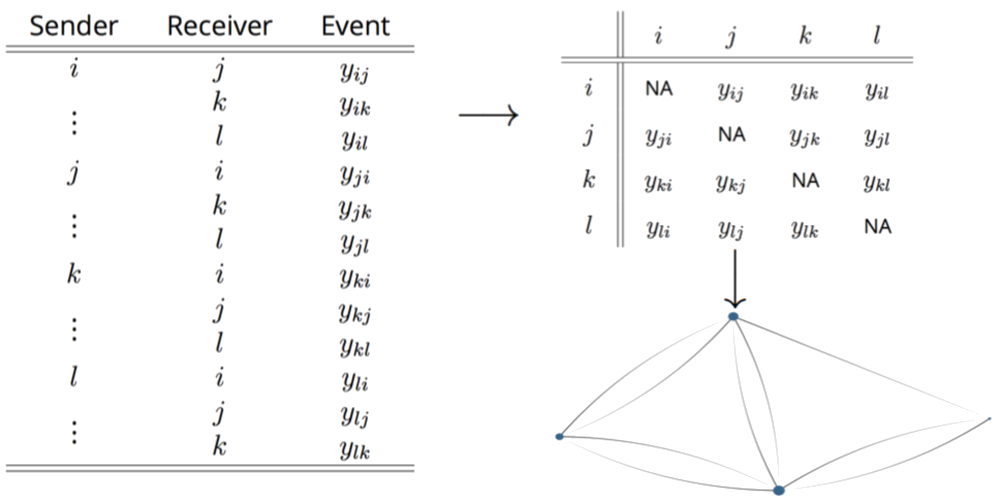
\includegraphics[width=1.05\textwidth]{df_adj_net3}
}
%%%%%%%%%%%%%%%%%%%%%%%%%%%%%%%%%%%%%%%%%%%%%%%%%%%%%%%%%%%%

%%%%%%%%%%%%%%%%%%%%%%%%%%%%%%%%%%%%%%%%%%%%%%%%%%%%%%%%%%%%
\frame{
  \frametitle{Relational data assumptions}

GLM: $y_{ij} \sim \beta^{T} X_{ij} + e_{ij}$

Networks typically show evidence against independence of {$e_{ij} : i \neq j$}

Not accounting for dependence can lead to:

\begin{itemize}
\item - biased effects estimation
\item - uncalibrated confidence intervals
\item - poor predictive performance
\item - inaccurate description of network phenomena
\end{itemize}

We've been hearing this concern for decades now:

\begin{tabular}{lll}
Thompson \& Walker (1982) & Beck et al. (1998) & Snijders (2011) \\
Frank \& Strauss (1986) & Signorino (1999) & Erikson et al. (2014) \\
Kenny (1996) & Li \& Loken (2002) & Aronow et al. (2015) \\
Krackhardt (1998) & Hoff \& Ward (2004) & Athey et al. (2016) \\
\end{tabular}

}
%%%%%%%%%%%%%%%%%%%%%%%%%%%%%%%%%%%%%%%%%%%%%%%%%%%%%%%%%%%%

%%%%%%%%%%%%%%%%%%%%%%%%%%%%%%%%%%%%%%%%%%%%%%%%%%%%%%%%%%%%
\frame{
  \frametitle{Outline}

\begin{itemize}
  \item - Nodal and dyadic dependencies in networks
  \item \qquad -  Can model using the ``A'' in AME 
  \item - Third order dependencies
  \item \qquad - Can model using the ``M'' in AME
  \item - Application
\end{itemize}

}
%%%%%%%%%%%%%%%%%%%%%%%%%%%%%%%%%%%%%%%%%%%%%%%%%%%%%%%%%%%%

%%%%%%%%%%%%%%%%%%%%%%%%%%%%%%%%%%%%%%%%%%%%%%%%%%%%%%%%%%%%
\frame{
  \frametitle{What network phenomena? Sender heterogeneity}

  Values across a row, say $\{y_{ij},y_{ik},y_{il}\}$, may be more similar to each other than other values in the adjacency matrix because each of these values has a common sender $i$

  \centering
  \includegraphics[width=.7\textwidth]{adjRowDep}

}
%%%%%%%%%%%%%%%%%%%%%%%%%%%%%%%%%%%%%%%%%%%%%%%%%%%%%%%%%%%%

%%%%%%%%%%%%%%%%%%%%%%%%%%%%%%%%%%%%%%%%%%%%%%%%%%%%%%%%%%%%
\frame{
  \frametitle{What network phenomena? Receiver heterogeneity}

  Values across a column, say $\{y_{ji},y_{ki},y_{li}\}$, may be more similar to each other than other values in the adjacency matrix because each of these values has a common receiver $i$

  \centering
  \includegraphics[width=.7\textwidth]{adjColDep}

}
%%%%%%%%%%%%%%%%%%%%%%%%%%%%%%%%%%%%%%%%%%%%%%%%%%%%%%%%%%%%

%%%%%%%%%%%%%%%%%%%%%%%%%%%%%%%%%%%%%%%%%%%%%%%%%%%%%%%%%%%%
\frame{
  \frametitle{What network phenomena? Sender-Receiver Covariance}

  Actors who are more likely to send ties in a network may also be more likely to receive them

  \centering
  \includegraphics[width=.7\textwidth]{adjRowColCovar}

}
%%%%%%%%%%%%%%%%%%%%%%%%%%%%%%%%%%%%%%%%%%%%%%%%%%%%%%%%%%%%

%%%%%%%%%%%%%%%%%%%%%%%%%%%%%%%%%%%%%%%%%%%%%%%%%%%%%%%%%%%%
\frame{
  \frametitle{What network phenomena? Reciprocity}

  Values of $y_{ij}$ and $y_{ji}$ may be statistically dependent

  \centering
  \includegraphics[width=.7\textwidth]{adjRecip}

}
%%%%%%%%%%%%%%%%%%%%%%%%%%%%%%%%%%%%%%%%%%%%%%%%%%%%%%%%%%%%

%%%%%%%%%%%%%%%%%%%%%%%%%%%%%%%%%%%%%%%%%%%%%%%%%%%%%%%%%%%%
\frame{
  \frametitle{Social Relations Model (The ``A'' in AME)}

We use this model to form the additive effects portion of AME

\begin{align*}
\begin{aligned}
      y_{ij} &= \color{red}{\mu} + \color{red}{e_{ij}} \\
      e_{ij} &= a_{i} + b_{j} + \epsilon_{ij} \\
      \{ (a_{1}, b_{1}), \ldots, (a_{n}, b_{n}) \} &\sim N(0,\Sigma_{ab}) \\ 
      \{ (\epsilon_{ij}, \epsilon_{ji}) : \; i \neq j\} &\sim N(0,\Sigma_{\epsilon}), \text{ where } \\
      \Sigma_{ab} = \begin{pmatrix} \sigma_{a}^{2} & \sigma_{ab} \\ \sigma_{ab} & \sigma_{b}^2   \end{pmatrix} \;\;\;\;\; &\Sigma_{\epsilon} = \sigma_{\epsilon}^{2} \begin{pmatrix} 1 & \rho \\ \rho & 1  \end{pmatrix}
\end{aligned}
\end{align*}

\begin{itemize}
\item - $\mu$ baseline measure of network activity
\item - $e_{ij}$ residual variation that we will use the SRM to decompose
\end{itemize}

}
%%%%%%%%%%%%%%%%%%%%%%%%%%%%%%%%%%%%%%%%%%%%%%%%%%%%%%%%%%%%

%%%%%%%%%%%%%%%%%%%%%%%%%%%%%%%%%%%%%%%%%%%%%%%%%%%%%%%%%%%%
\frame{
  \frametitle{Social Relations Model (The ``A'' in AME)}

\begin{align*}
\begin{aligned}
      y_{ij} &= \mu + e_{ij} \\
      e_{ij} &= \color{red}{a_{i} + b_{j}} + \epsilon_{ij} \\
      \color{red}{\{ (a_{1}, b_{1}), \ldots, (a_{n}, b_{n}) \}} &\sim N(0,\Sigma_{ab}) \\ 
      \{ (\epsilon_{ij}, \epsilon_{ji}) : \; i \neq j\} &\sim N(0,\Sigma_{\epsilon}), \text{ where } \\
      \Sigma_{ab} = \begin{pmatrix} \sigma_{a}^{2} & \sigma_{ab} \\ \sigma_{ab} & \sigma_{b}^2   \end{pmatrix} \;\;\;\;\; &\Sigma_{\epsilon} = \sigma_{\epsilon}^{2} \begin{pmatrix} 1 & \rho \\ \rho & 1  \end{pmatrix}
\end{aligned}
\end{align*}

\begin{itemize}
\item - row/sender effect ($a_{i}$) \& column/receiver effect ($b_{j}$)
\item - Modeled jointly to account for correlation in how active an actor is in sending and receiving ties
\end{itemize}

}
%%%%%%%%%%%%%%%%%%%%%%%%%%%%%%%%%%%%%%%%%%%%%%%%%%%%%%%%%%%%

%%%%%%%%%%%%%%%%%%%%%%%%%%%%%%%%%%%%%%%%%%%%%%%%%%%%%%%%%%%%
\frame{
  \frametitle{Social Relations Model (The ``A'' in AME)}

\begin{align*}
\begin{aligned}
      y_{ij} &= \mu + e_{ij} \\
      e_{ij} &= a_{i} + b_{j} + \epsilon_{ij} \\
      \{ (a_{1}, b_{1}), \ldots, (a_{n}, b_{n}) \} &\sim N(0,\color{red}{\Sigma_{ab}}) \\ 
      \{ (\epsilon_{ij}, \epsilon_{ji}) : \; i \neq j\} &\sim N(0,\Sigma_{\epsilon}), \text{ where } \\
      \color{red}{\Sigma_{ab}} = \begin{pmatrix} \sigma_{a}^{2} & \sigma_{ab} \\ \sigma_{ab} & \sigma_{b}^2   \end{pmatrix} \;\;\;\;\; &\Sigma_{\epsilon} = \sigma_{\epsilon}^{2} \begin{pmatrix} 1 & \rho \\ \rho & 1  \end{pmatrix}
\end{aligned}
\end{align*}

\begin{itemize}
\item - $\sigma_{a}^{2}$ and $\sigma_{b}^{2}$ capture heterogeneity in the row and column means
\item - $\sigma_{ab}$ describes the linear relationship between these two effects (i.e., whether actors who send [receive] a lot of ties also receive [send] a lot of ties)
\end{itemize}

}
%%%%%%%%%%%%%%%%%%%%%%%%%%%%%%%%%%%%%%%%%%%%%%%%%%%%%%%%%%%%

%%%%%%%%%%%%%%%%%%%%%%%%%%%%%%%%%%%%%%%%%%%%%%%%%%%%%%%%%%%%
\frame{
  \frametitle{Social Relations Model (The ``A'' in AME)}

\begin{align*}
\begin{aligned}
      y_{ij} &= \mu + e_{ij} \\
      e_{ij} &= a_{i} + b_{j} + \color{red}{\epsilon_{ij}} \\
      \{ (a_{1}, b_{1}), \ldots, (a_{n}, b_{n}) \} &\sim N(0,\Sigma_{ab}) \\ 
      \color{red}{\{ (\epsilon_{ij}, \epsilon_{ji}) : \; i \neq j\}} &\sim N(0,\color{red}{\Sigma_{\epsilon}}), \text{ where } \\
      \Sigma_{ab} = \begin{pmatrix} \sigma_{a}^{2} & \sigma_{ab} \\ \sigma_{ab} & \sigma_{b}^2   \end{pmatrix} \;\;\;\;\; & \color{red}{\Sigma_{\epsilon}} = \sigma_{\epsilon}^{2} \begin{pmatrix} 1 & \rho \\ \rho & 1  \end{pmatrix}
\end{aligned}
\end{align*}

\begin{itemize}
\item - $\epsilon_{ij}$ captures the within dyad effect
\item - Second-order dependencies are described by $\sigma_{\epsilon}^{2}$
\item - Reciprocity, aka within dyad correlation, represented by $\rho$
\end{itemize}
}
%%%%%%%%%%%%%%%%%%%%%%%%%%%%%%%%%%%%%%%%%%%%%%%%%%%%%%%%%%%%

%%%%%%%%%%%%%%%%%%%%%%%%%%%%%%%%%%%%%%%%%%%%%%%%%%%%%%%%%%%%
\frame{
  \frametitle{Third Order Dependencies}

  \vspace{-10mm}

  \begin{table}[ht]
  \begin{tabular}{lcr}
  \scshape{Homophily} & & \scshape{Stochastic Equivalence} \\
  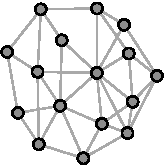
\includegraphics[width=.33\textwidth]{homophNet} & \hspace{2cm} &
  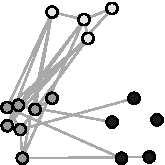
\includegraphics[width=.33\textwidth]{stochEquivNet}  
  \end{tabular}
  \end{table}

  To account for these patterns we can build on what we have so far and find an expression for $\gamma$:
  
  \vspace{-5mm}
  \begin{align*}
  \centering
  y_{ij} &\approx \beta^{T} X_{ij} + a_{i} + b_{j} + \gamma(u_{i},v_{j})
  \end{align*}

}
%%%%%%%%%%%%%%%%%%%%%%%%%%%%%%%%%%%%%%%%%%%%%%%%%%%%%%%%%%%%

%%%%%%%%%%%%%%%%%%%%%%%%%%%%%%%%%%%%%%%%%%%%%%%%%%%%%%%%%%%%
\frame{
  \frametitle{Latent Factor Model: The ``M'' in AME}

Each node $i$ has an unknown latent factor

\vspace{-5mm}
\begin{align*}
{\textbf{u}_{i},\textbf{v}_{j}} \in \mathbb{R}^{k} \;\; i,j \in \{1, \ldots, n \} \\
\end{align*}

\vspace{-5mm}
The probability of a tie from $i$ to $j$ depends on their latent factors

\vspace{-5mm}
\begin{align*}
\begin{aligned}
  \gamma(\textbf{u}_{i}, \textbf{v}_{j}) &= \textbf{u}_{i}^{T} D \textbf{v}_{j} \\
  &= \sum_{k \in K} d_{k} u_{ik} v_{jk} \\
  &D \text{ is a  } K \times K \text{ diagonal matrix}
\end{aligned}
\end{align*}

Can account for both stochastic equivalence and homophily

}
%%%%%%%%%%%%%%%%%%%%%%%%%%%%%%%%%%%%%%%%%%%%%%%%%%%%%%%%%%%%

%%%%%%%%%%%%%%%%%%%%%%%%%%%%%%%%%%%%%%%%%%%%%%%%%%%%%%%%%%%%
\frame{
  \frametitle{Swiss Climate Change Application}

Cross-sectional network measuring whether an actor indicated that they collaborated with another during the policy design of the Swiss CO$_{2}$ act (Ingold 2008)

\begin{figure}[ht]
  \centering
  \begin{tabular}{cc}
  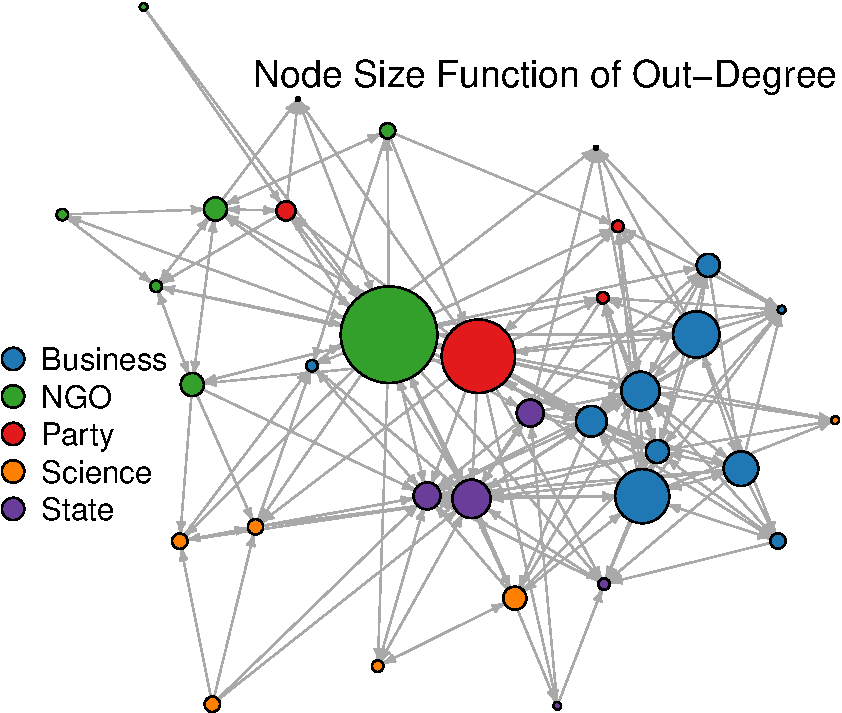
\includegraphics[width=.47\textwidth]{dvNet_outDegree} & 
  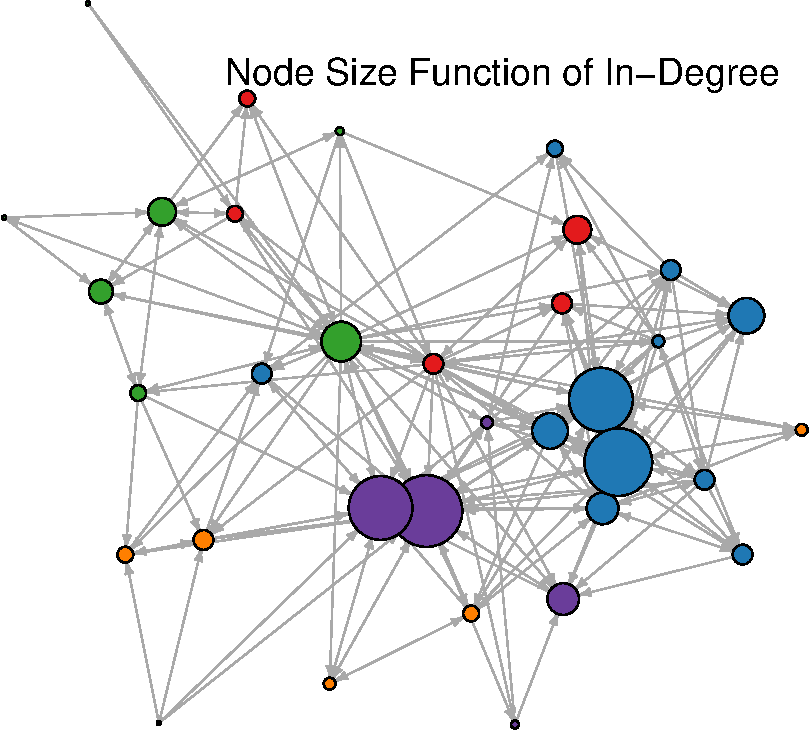
\includegraphics[width=.44\textwidth]{dvNet_inDegree}
  \end{tabular}
\end{figure}

}
%%%%%%%%%%%%%%%%%%%%%%%%%%%%%%%%%%%%%%%%%%%%%%%%%%%%%%%%%%%%

%%%%%%%%%%%%%%%%%%%%%%%%%%%%%%%%%%%%%%%%%%%%%%%%%%%%%%%%%%%%
\frame{
  \frametitle{Parameter Estimates}

% latex table generated in R 3.3.1 by xtable 1.8-2 package
% Sun Aug 21 03:32:43 2016
\vspace{-15mm}
\begin{table}[ht]
\centering
\begingroup\scriptsize
\begin{tabular}{lcccccc}
   & Expected & \multirow{2}{*}{Logit} & \multirow{2}{*}{MRQAP} & \multirow{2}{*}{LSM} & \multirow{2}{*}{ERGM} & \multirow{2}{*}{AME} \\ 
   & Effect & & & & & \\
  \hline
  \textbf{Conflicting policy preferences} &  &  &  &  &  &  \\ 
  $\;\;\;\;$ Business vs. NGO & \color{red}{$-$} & -0.86 & \color{red}{-0.87$^{\ast}$} & \color{red}{-1.37$^{\ast}$} & \color{red}{-1.11$^{\ast}$} & \color{red}{-1.37$^{\ast}$} \\ 
  $\;\;\;\;$ Opposition/alliance & \color{blue}{$+$} &  \color{blue}{1.21$^{\ast}$} & \color{blue}{1.14$^{\ast}$} & 0.00 & \color{blue}{1.22$^{\ast}$} & \color{blue}{1.08$^{\ast}$} \\ 
  $\;\;\;\;$ Preference dissimilarity & \color{red}{$-$} & -0.07 & -0.60 & \color{red}{-1.76$^{\ast}$} & -0.44 & \color{red}{-0.79$^{\ast}$} \\ 
  \textbf{Transaction costs} &  &  &  &  &  &  \\ 
  $\;\;\;\;$ Joint forum participation & \color{blue}{$+$} & \color{blue}{0.88$^{\ast}$} & \color{blue}{0.75$^{\ast}$} & \color{blue}{1.51$^{\ast}$} & \color{blue}{0.90$^{\ast}$} & \color{blue}{0.92$^{\ast}$} \\ 
  \textbf{Influence} & &  &  &  &  &  \\ 
  $\;\;\;\;$ Influence attribution & \color{blue}{$+$} & \color{blue}{1.20$^{\ast}$} & \color{blue}{1.29$^{\ast}$} & 0.08 & \color{blue}{1.00$^{\ast}$} & \color{blue}{1.09$^{\ast}$} \\ 
  $\;\;\;\;$ Alter's influence indegree & \color{blue}{$+$} & \color{blue}{0.10$^{\ast}$} & \color{blue}{0.11$^{\ast}$} & 0.01 & \color{blue}{0.21$^{\ast}$} & \color{blue}{0.11$^{\ast}$} \\ 
  $\;\;\;\;$ Influence absolute diff. & \color{red}{$-$} & \color{red}{-0.03$^{\ast}$} & \color{red}{-0.06$^{\ast}$} & 0.04 & \color{red}{-0.05$^{\ast}$} & \color{red}{-0.07$^{\ast}$} \\ 
  $\;\;\;\;$ Alter = Government actor & \color{blue}{$+$} & \color{blue}{0.63$^{\ast}$} & 0.68 & -0.46 & \color{blue}{1.04$^{\ast}$} & 0.55 \\ 
  \textbf{Functional requirements} &  &  &  &  &  & \\ 
  $\;\;\;\;$ Ego = Environmental NGO & \color{blue}{$+$} & \color{blue}{0.88$^{\ast}$} & 0.99 & -0.60 & \color{blue}{0.79$^{\ast}$} & 0.67 \\ 
  $\;\;\;\;$ Same actor type & \color{blue}{$+$} & \color{blue}{0.74$^{\ast}$} & \color{blue}{1.12$^{\ast}$} & \color{blue}{1.17$^{\ast}$} & \color{blue}{0.99$^{\ast}$} & \color{blue}{1.04$^{\ast}$} \\ 
   \hline
\end{tabular}
\endgroup
\end{table}

}
%%%%%%%%%%%%%%%%%%%%%%%%%%%%%%%%%%%%%%%%%%%%%%%%%%%%%%%%%%%%

%%%%%%%%%%%%%%%%%%%%%%%%%%%%%%%%%%%%%%%%%%%%%%%%%%%%%%%%%%%%
\frame{
  \frametitle{Latent Factor Visualization}

  \centering
  \vspace{-10mm}
  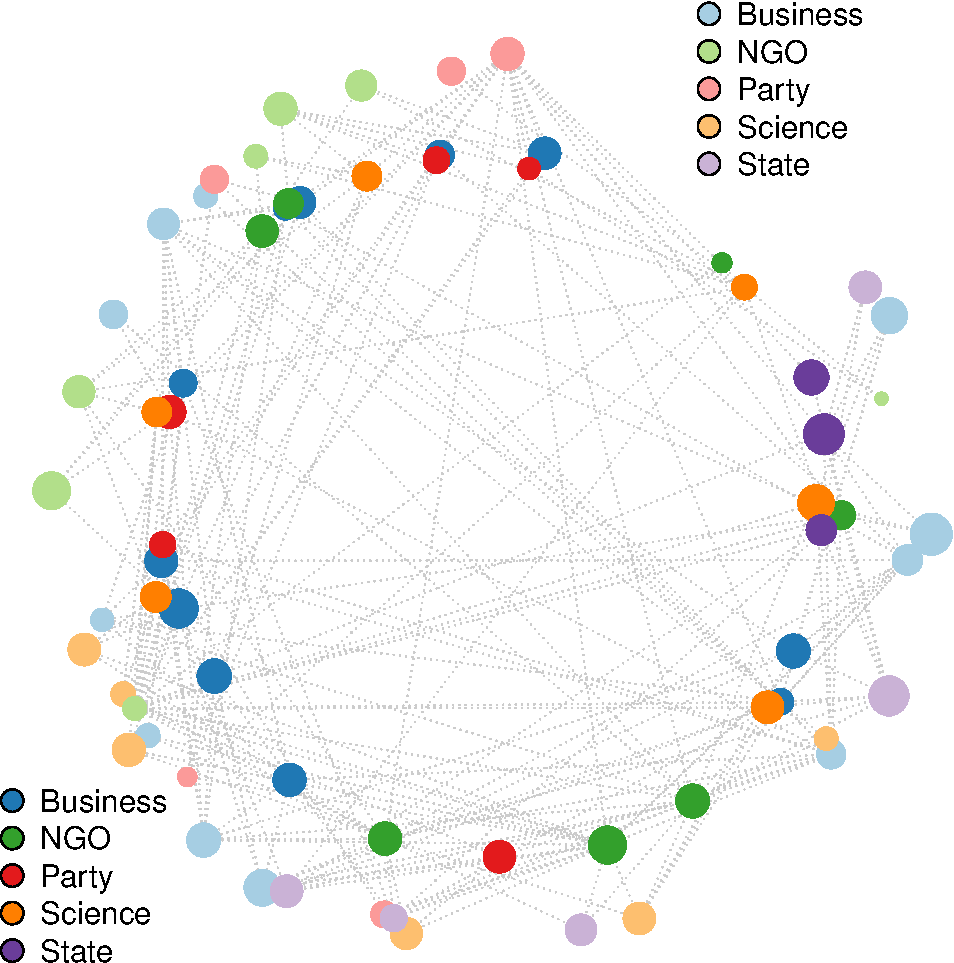
\includegraphics[width=.7\textwidth]{ameFitSR_2_UV}

}
%%%%%%%%%%%%%%%%%%%%%%%%%%%%%%%%%%%%%%%%%%%%%%%%%%%%%%%%%%%%

%%%%%%%%%%%%%%%%%%%%%%%%%%%%%%%%%%%%%%%%%%%%%%%%%%%%%%%%%%%%
\frame{
  \frametitle{Out of Sample Performance Assessment}

\begin{itemize}
  \item - Randomly divide the $n \times (n-1)$ data points into $S$ sets of roughly equal size, letting $s_{ij}$ be the set to which pair $\{ij\}$ is assigned.
  \item - For each $s \in \{1, \ldots, S\}$:
  \begin{itemize}
    \item - Obtain estimates of the model parameters conditional on $\{y_{ij} : s_{ij} \neq s\}$, the data on pairs not in set $s$.
    \item - For pairs $\{kl\}$ in set $s$, let $\hat y_{kl} = E[y_{kl} | \{y_{ij} : s_{ij} \neq s\}]$, the predicted value of $y_{kl}$ obtained using data not in set $s$.
  \end{itemize}
\end{itemize}

This procedure generates a sociomatrix of out-of-sample predictions of the observed data

}
%%%%%%%%%%%%%%%%%%%%%%%%%%%%%%%%%%%%%%%%%%%%%%%%%%%%%%%%%%%%

%%%%%%%%%%%%%%%%%%%%%%%%%%%%%%%%%%%%%%%%%%%%%%%%%%%%%%%%%%%%
\frame{
  \frametitle{Performance Comparison}

\begin{tabular}{cc}
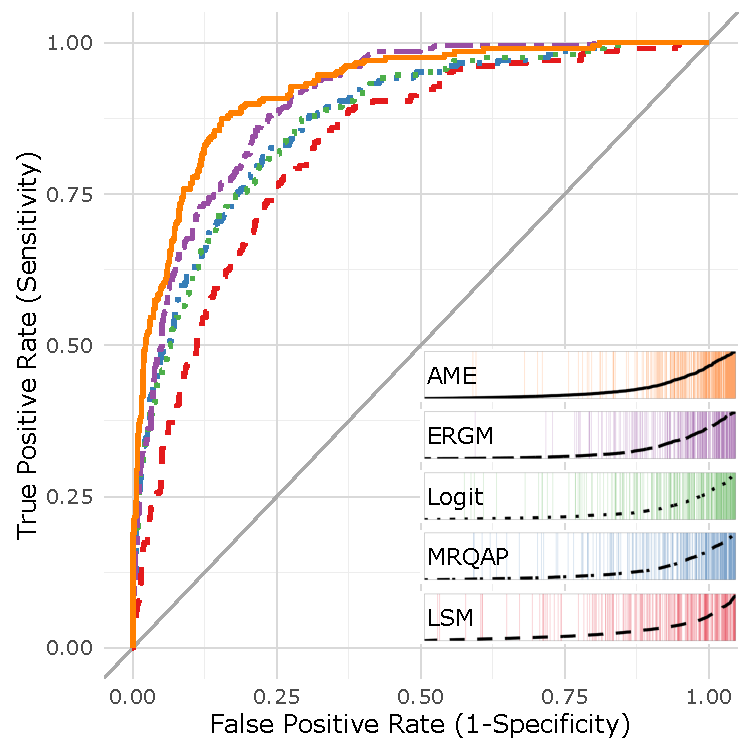
\includegraphics[width=.5\textwidth]{roc_outSample} & 
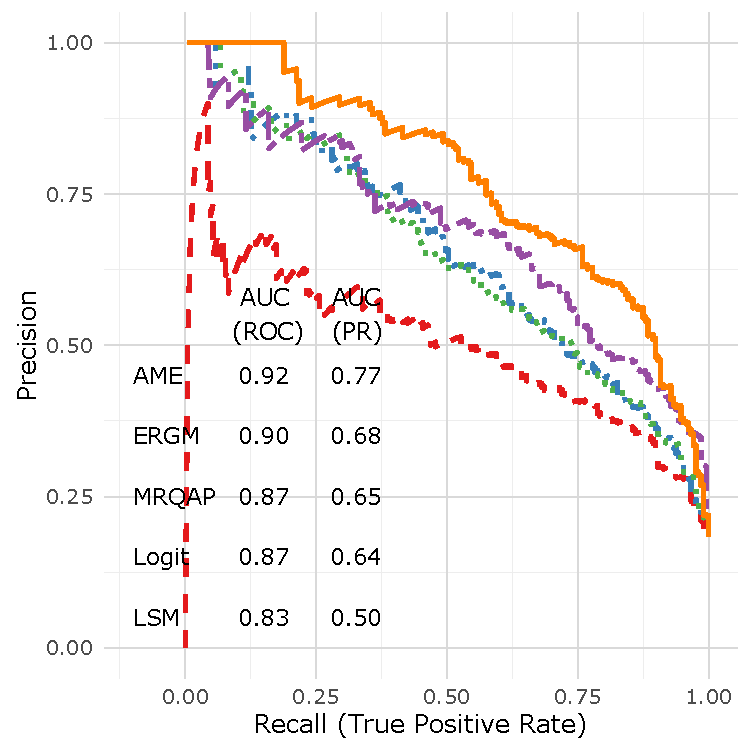
\includegraphics[width=.5\textwidth]{rocPr_outSample} 
\end{tabular}

}
%%%%%%%%%%%%%%%%%%%%%%%%%%%%%%%%%%%%%%%%%%%%%%%%%%%%%%%%%%%%

%%%%%%%%%%%%%%%%%%%%%%%%%%%%%%%%%%%%%%%%%%%%%%%%%%%%%%%%%%%%
\frame{
  \frametitle{Network Dependencies}


  \centering
  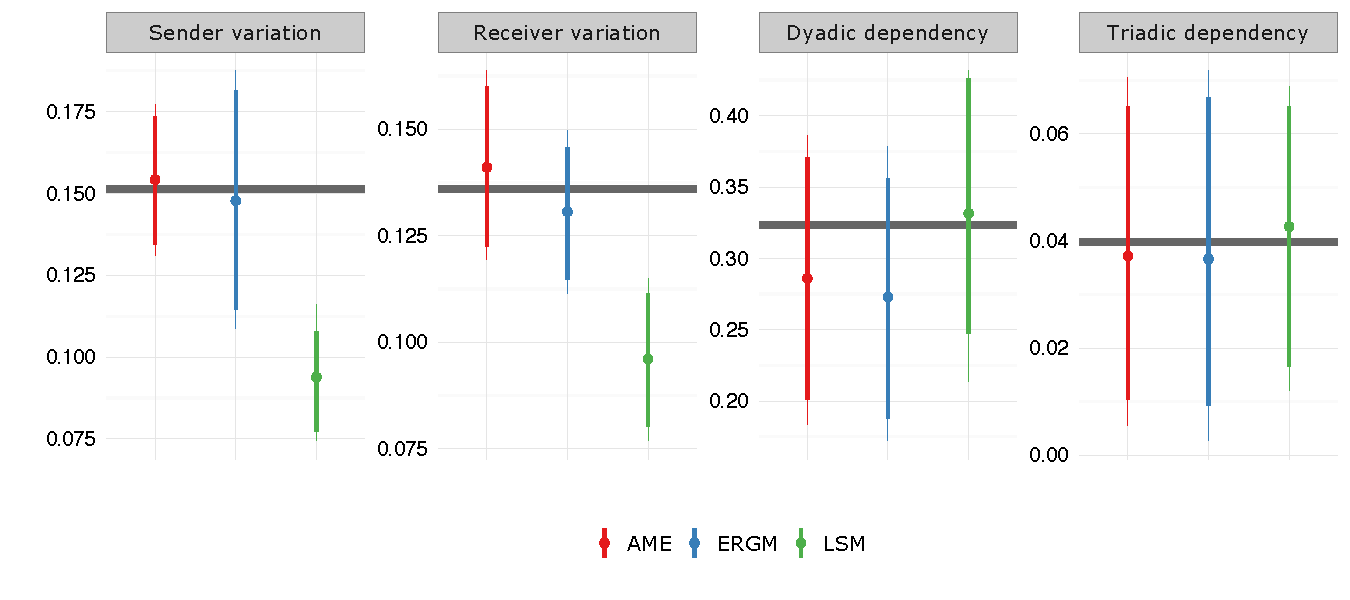
\includegraphics[width=1\textwidth]{netPerfCoef}

}
%%%%%%%%%%%%%%%%%%%%%%%%%%%%%%%%%%%%%%%%%%%%%%%%%%%%%%%%%%%%

%%%%%%%%%%%%%%%%%%%%%%%%%%%%%%%%%%%%%%%%%%%%%%%%%%%%%%%%%%%%
\frame{
  \frametitle{What's Next?}

  \begin{itemize}
    \item - Extending AMEN to handle changing actor compositions
    \item - Generalize multiplicative effects estimation over tensors
  \end{itemize}

}
%%%%%%%%%%%%%%%%%%%%%%%%%%%%%%%%%%%%%%%%%%%%%%%%%%%%%%%%%%%%

%%%%%%%%%%%%%%%%%%%%%%%%%%%%%%%%%%%%%%%%%%%%%%%%%%%%%%%%%%%%
\plain{Thanks.}
%%%%%%%%%%%%%%%%%%%%%%%%%%%%%%%%%%%%%%%%%%%%%%%%%%%%%%%%%%%%

%%%%%%%%%%%%%%%%%%%%%%%%%%%%%%%%%%%%%%%%%%%%%%%%%%%%%%%%%%%%
\frame{
  \frametitle{Standard Network Dependence Measures}
\vspace{-5mm}
\includegraphics[width=1\textwidth]{ggGofAll_preeze}
}
%%%%%%%%%%%%%%%%%%%%%%%%%%%%%%%%%%%%%%%%%%%%%%%%%%%%%%%%%%%%

%%%%%%%%%%%%%%%%%%%%%%%%%%%%%%%%%%%%%%%%%%%%%%%%%%%%%%%%%%%%
\frame{
  \frametitle{Simulation Comparison}

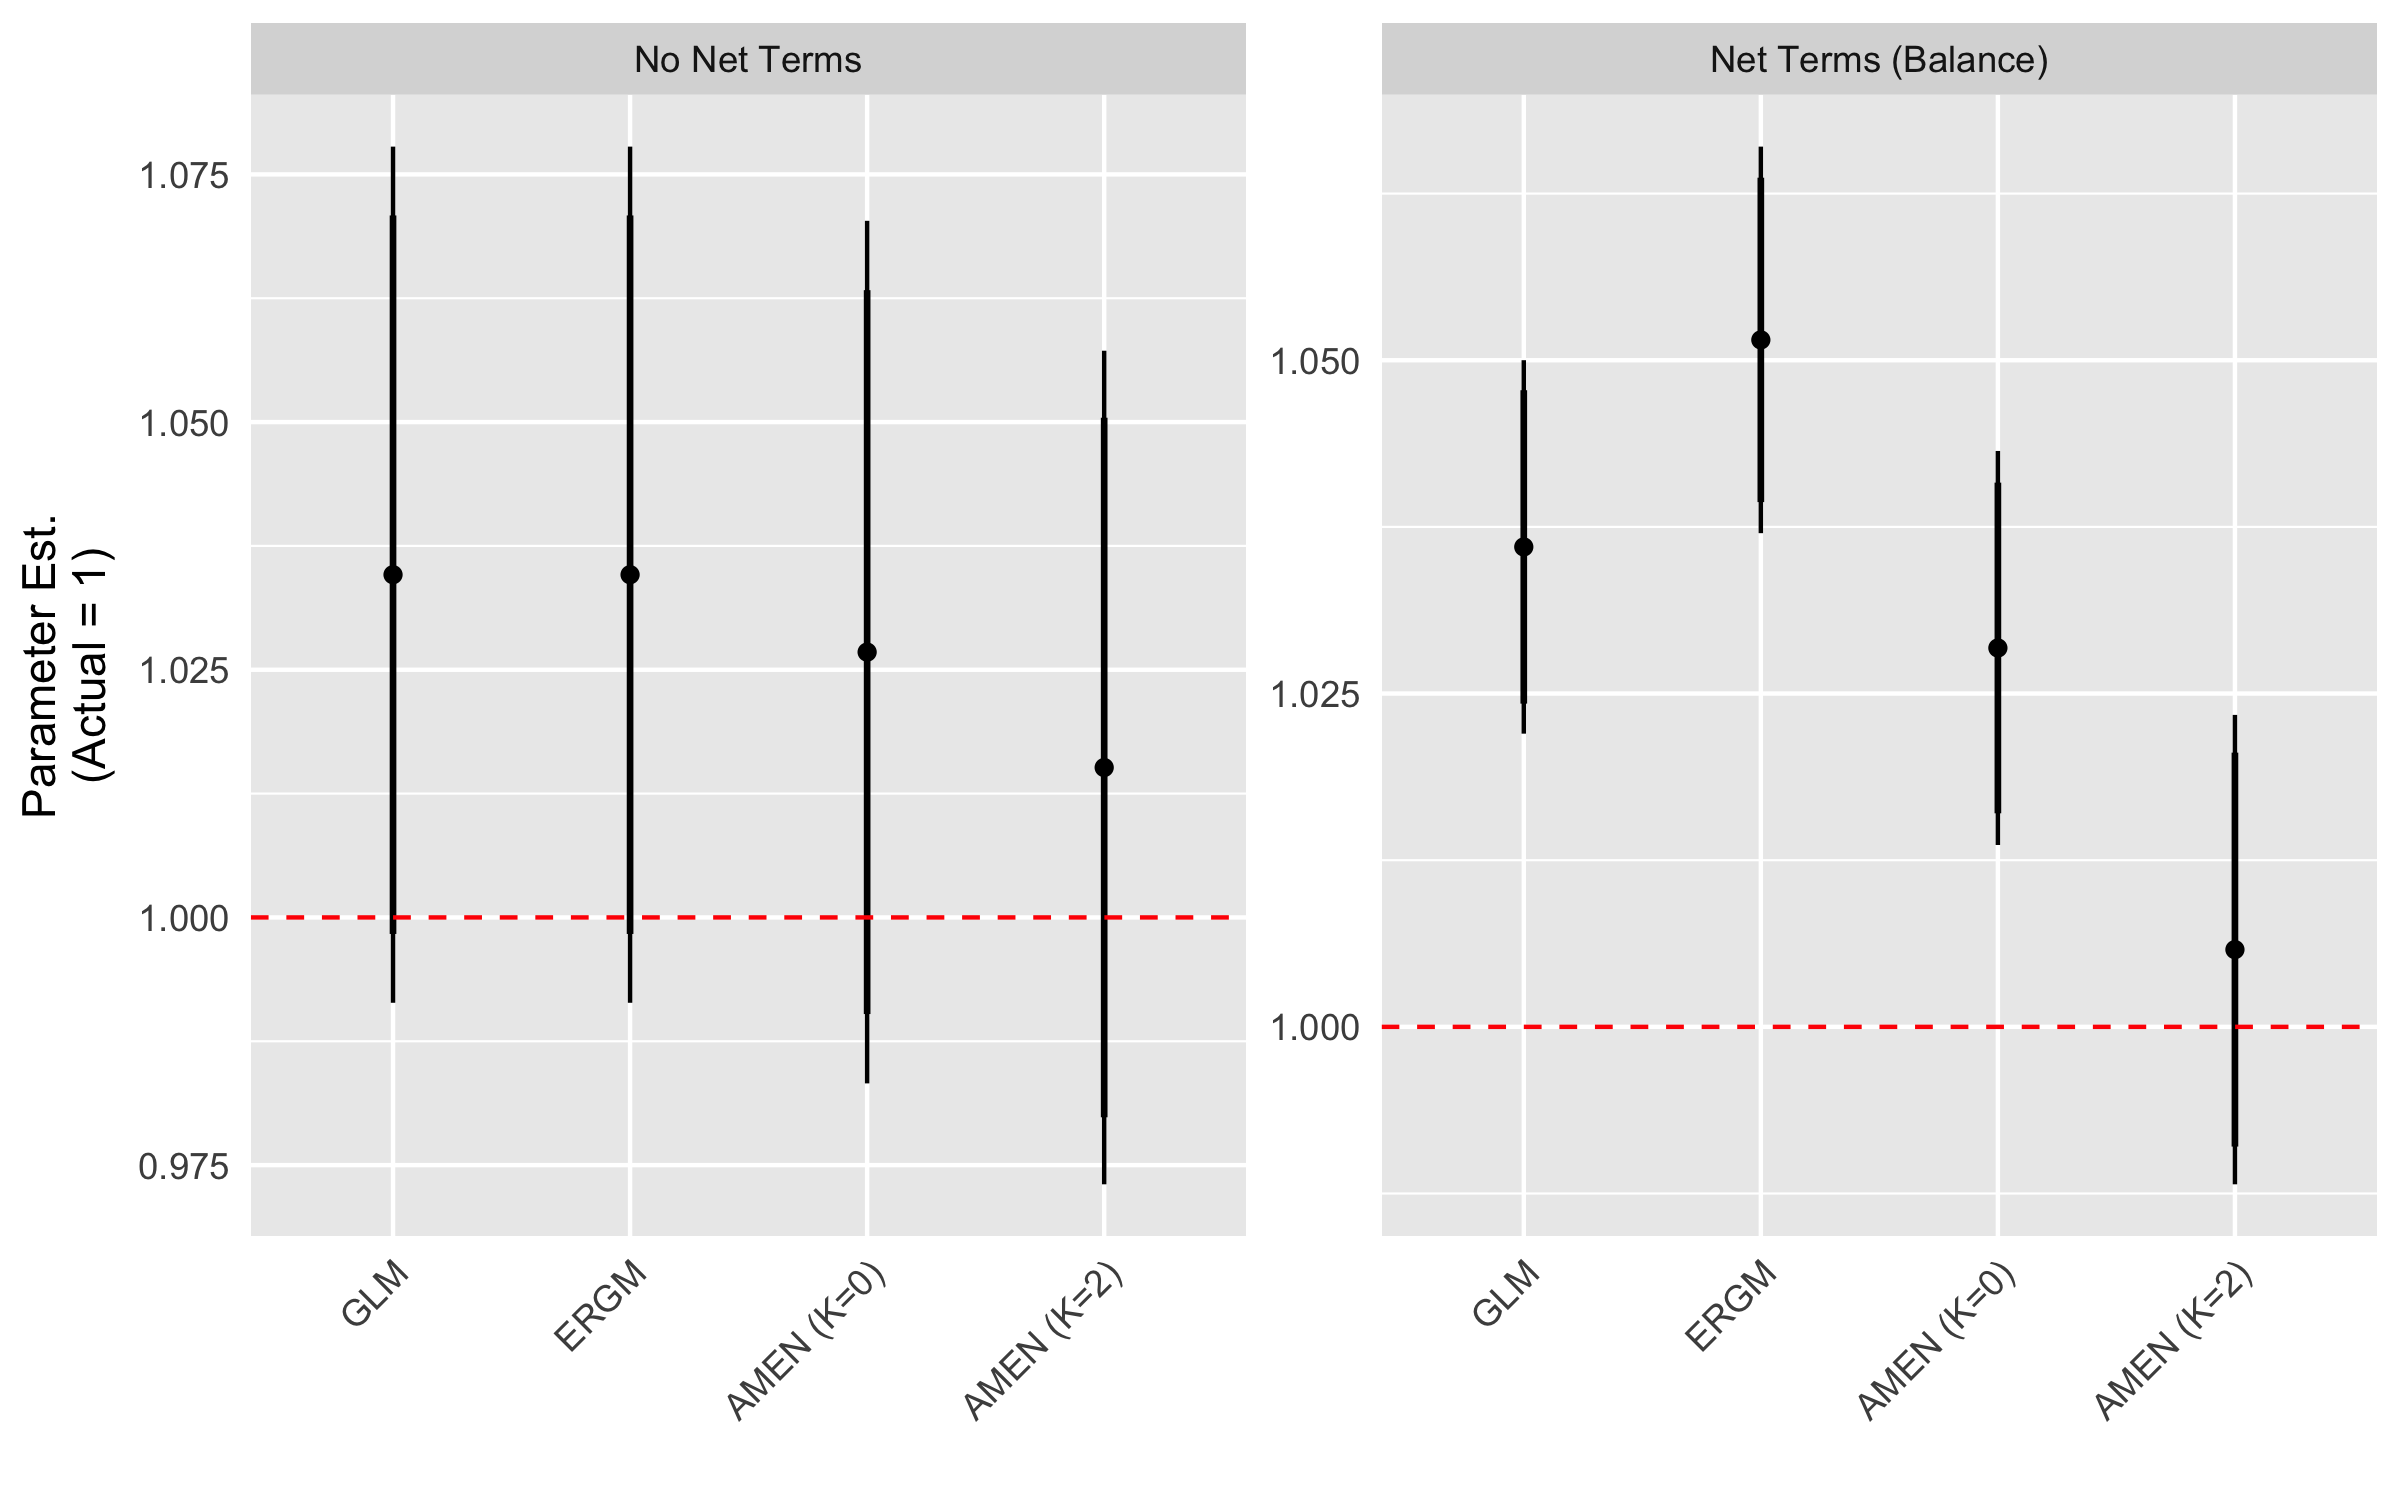
\includegraphics[width=1\textwidth]{ameVergmSim.png}

}
%%%%%%%%%%%%%%%%%%%%%%%%%%%%%%%%%%%%%%%%%%%%%%%%%%%%%%%%%%%%

%%%%%%%%%%%%%%%%%%%%%%%%%%%%%%%%%%%%%%%%%%%%%%%%%%%%%%%%%%%%
\frame{
  \frametitle{AMEN v LSM Performance}

  \begin{tabular}{cc}
  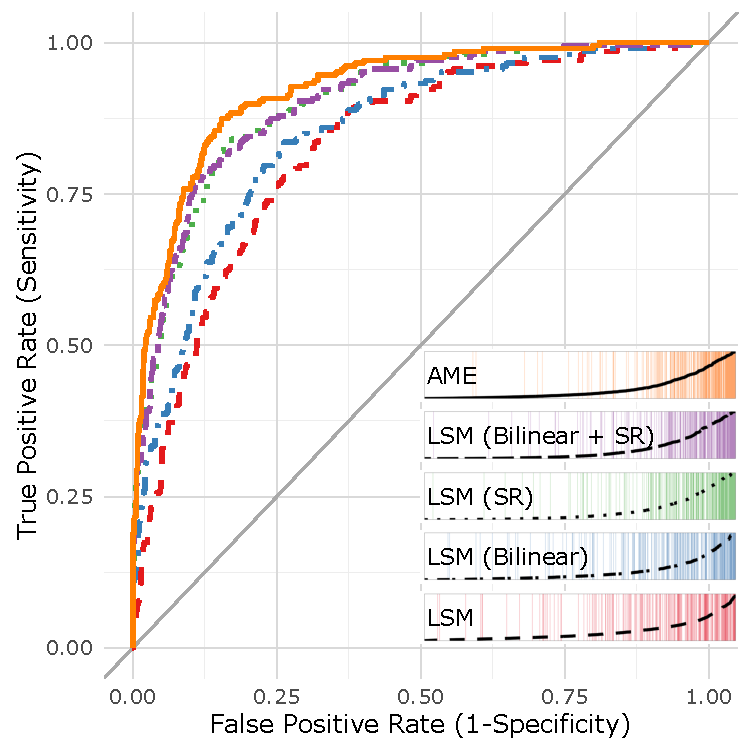
\includegraphics[width=.5\textwidth]{roc_latSpace_outSample} & 
  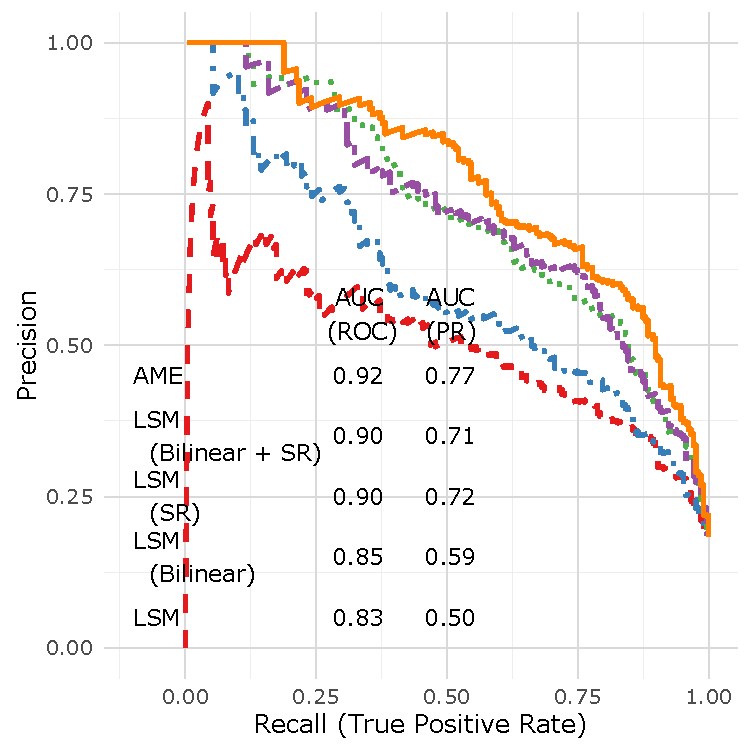
\includegraphics[width=.5\textwidth]{rocPr_latSpace_outSample}
  \end{tabular}

}
%%%%%%%%%%%%%%%%%%%%%%%%%%%%%%%%%%%%%%%%%%%%%%%%%%%%%%%%%%%%

%%%%%%%%%%%%%%%%%%%%%%%%%%%%%%%%%%%%%%%%%%%%%%%%%%%%%%%%%%%%
\frame{
  \frametitle{AMEN versus LSM Net Dependence}

  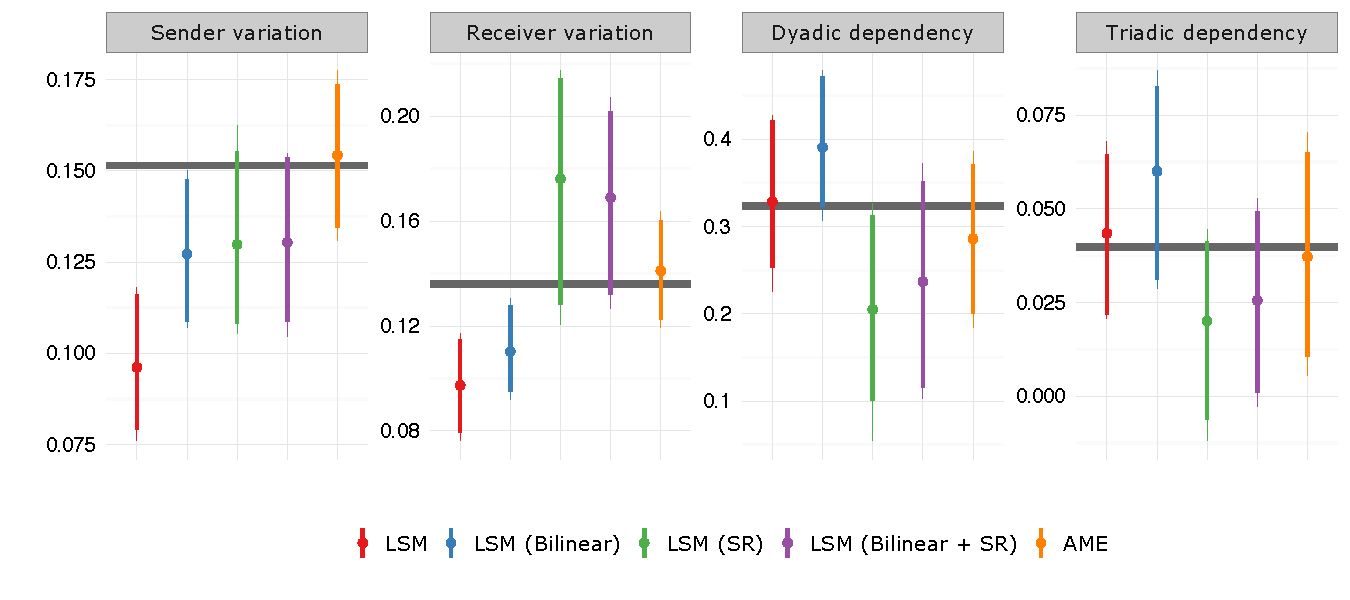
\includegraphics[width=1\textwidth]{netPerfCoef_latSpace}
}
%%%%%%%%%%%%%%%%%%%%%%%%%%%%%%%%%%%%%%%%%%%%%%%%%%%%%%%%%%%%

%%%%%%%%%%%%%%%%%%%%%%%%%%%%%%%%%%%%%%%%%%%%%%%%%%%%%%%%%%%%
\frame{
  \frametitle{AMEN varying $K$ Performance}

  \begin{tabular}{cc}
  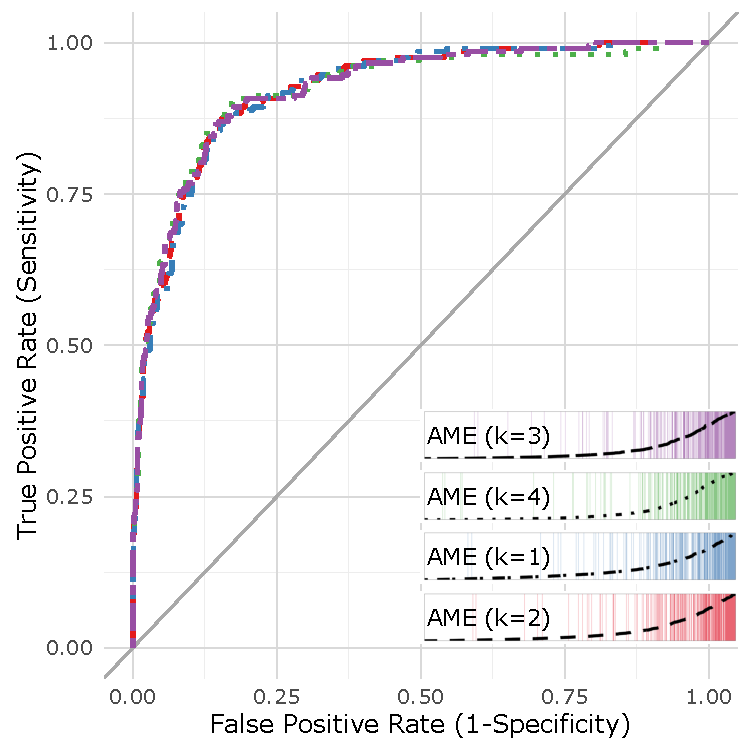
\includegraphics[width=.5\textwidth]{roc_ameSR_outSample} & 
  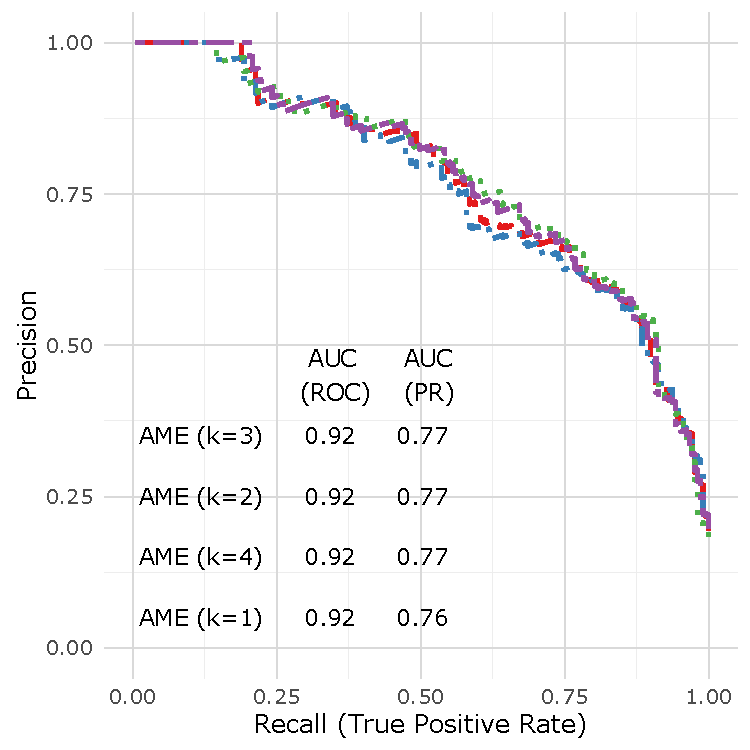
\includegraphics[width=.5\textwidth]{rocPr_ameSR_outSample}
  \end{tabular}

}
%%%%%%%%%%%%%%%%%%%%%%%%%%%%%%%%%%%%%%%%%%%%%%%%%%%%%%%%%%%%

%%%%%%%%%%%%%%%%%%%%%%%%%%%%%%%%%%%%%%%%%%%%%%%%%%%%%%%%%%%%
\frame{
  \frametitle{AMEN varying $K$ Net Dependence}

  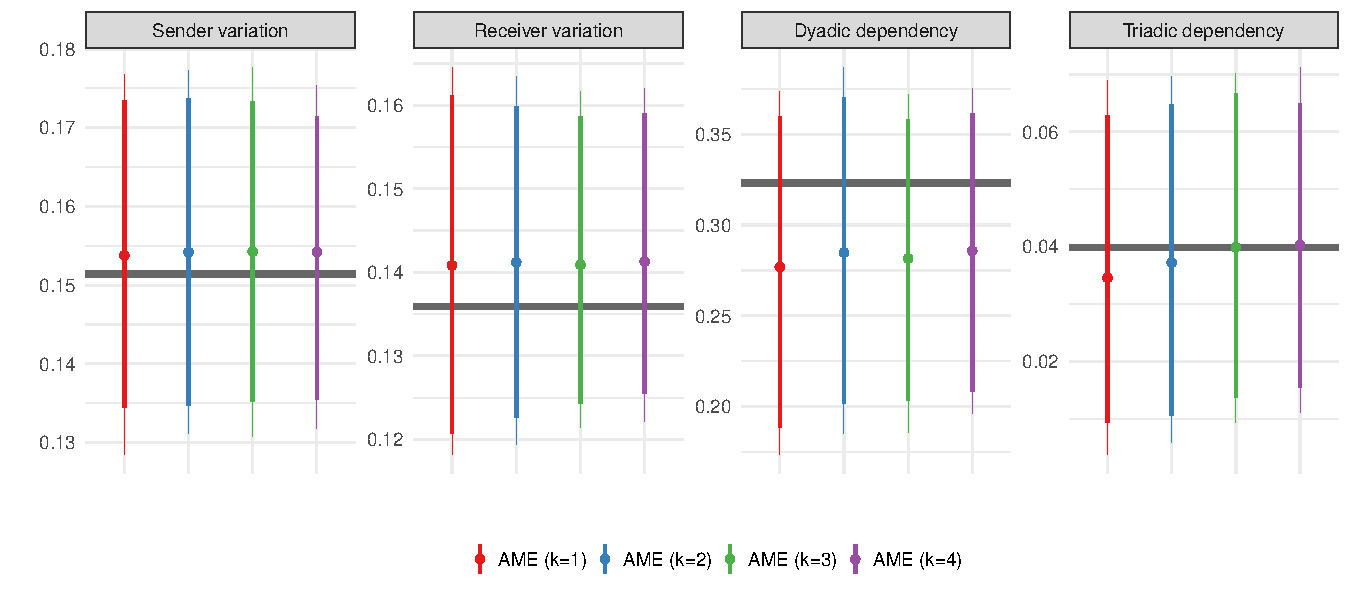
\includegraphics[width=1\textwidth]{netPerfCoef_ameSR}
}
%%%%%%%%%%%%%%%%%%%%%%%%%%%%%%%%%%%%%%%%%%%%%%%%%%%%%%%%%%%%

\end{document}
